\documentclass[hyperref, UTF8
,bookmarksnumbered=true, oneside]{ctexbook}
\hypersetup{
            bookmarksnumbered=true,
            bookmarksopen=true,
            colorlinks=false, 
            pdfborder=001,   
				%menucolor=green,%uunknown
				linktocpage=true,%make the link of the content on the number of page
            linkcolor=green,
            anchorcolor=green,
            citecolor=green}
\usepackage{geometry}
\usepackage{tocbibind}
\usepackage{graphicx}
\usepackage{amsmath}
\usepackage{amsfonts}
\usepackage{amssymb}
\usepackage{bm}
\CTEXsetup[name={(,)}]{chapter}
%\CTEXsetup[number={\chinese{section}}]{section}


\newcommand{\beqt}{\begin{equation}}
\newcommand{\eeqt}{\end{equation}}
\newcommand{\beqtnt}{\begin{equation*}}
\newcommand{\eeqtnt}{\end{equation*}}

\geometry{a4paper,centering,scale=0.8}

\title{\huge{软件工程课程作业}\\ \Huge \textbf{Mathematica Input Assistant} \\\phantom{aaa} \\\Huge{测试文档}}
\author{\\ \phantom{aaa} \\\phantom{aaa} \\ \phantom{aaa}\\\\\\\huge{待定小组}\\\\ \Large{基科物理32{  }蒋文韬}\\ \Large{基科物理32{ }张思源{ }}\\ \Large{基科应用31{  }李泽清{ }} \\ \Large{基科应用31 { }傅笛{ }} }
\begin{document}\Large

\frontmatter
\maketitle

\tableofcontents

\mainmatter

\chapter{测试规划及说明}

	\section{测试说明} % (fold)

		\subsection{功能测试} % (fold)
软件功能主要包括使用函数、添加函数和搜索函数这三个功能,于是按照这三个功能进行单元测试。另外,还要对整个软件的外观可操作部分点击功能进行集成测试。
		
		% subsection 功能测试 (end)

		\subsection{压力测试} % (fold)
因为根据软件功能需要,并不需要生成很大的Mathematica的代码,所以整个软件并不面临极大的压力测试。
		
		% subsection 压力测试 (end)
		
	% section 测试说明 (end)

	\section{测试内容} % (fold)
首先对Mathematica Input Assistant软件的外观功能进行集成测试,然后对该软件单元测试内容主要包括:使用函数、添加和删除函数和函数类,以及搜索函数这三个功能,在测试内容及展示中将详细说明。
	
	% section 测试内容 (end)

	\section{测试环境} % (fold)
		\begin{itemize}
			\item Windows 10
			\item Java runtime environment jre1.8.0\_60
		\end{itemize}
	
	% section 测试环境 (end)

	\section{测试工具} % (fold)
		\begin{itemize}
			\item 手动测试
			\item 黑盒测试
		\end{itemize}
	
	% section 测试工具 (end)

	\section{测试用例} % (fold)
		\begin{itemize}
			\item 表观测试
				\begin{itemize}
					\item 欢迎界面测试
					\item 菜单栏子目录显示、左侧树形结构窗口按钮以及滚动条使用测试
					\item 子对话框的显示
					\item 右侧操作窗口按钮测试
				\end{itemize}
			\item 函数使用测试
				\begin{itemize}
					\item ParametricPlot
					\item ContourPlot3D
				\end{itemize}
			\item 函数和函数类添加测试
				\begin{itemize}
					\item PolarPlot
				\end{itemize}
			\item 搜索函数功能测试
				\begin{itemize}
					\item 搜索框弹出测试
					\item 即时反应检索功能测试
					\item 搜索对话框按钮测试
				\end{itemize}
			\item 细节功能测试
				\begin{itemize}
					\item 函数名称输入非法测试
					\item 步长选择提示测试
					\item 函数函数类删除操作测试
				\end{itemize}
		\end{itemize}
	
	% section 测试用例 (end)


\chapter{测试内容及展示}

	\section{表观测试} % (fold)
		\subsection{欢迎界面测试:} % (fold)
		\begin{itemize}
			\item 用例名称: 欢迎界面测试
			\item 用例描述: 欢迎界面显示,左侧树形结构全部收起,菜单栏子菜单不显示。
			\item 测试过程: 双击程序图标将软件打开。
			\item 预计结果: 欢迎界面按预期完整显示。
			\item 测试结果:	和预期结果相一致。

				\begin{figure}[!h]
                	\centering
                	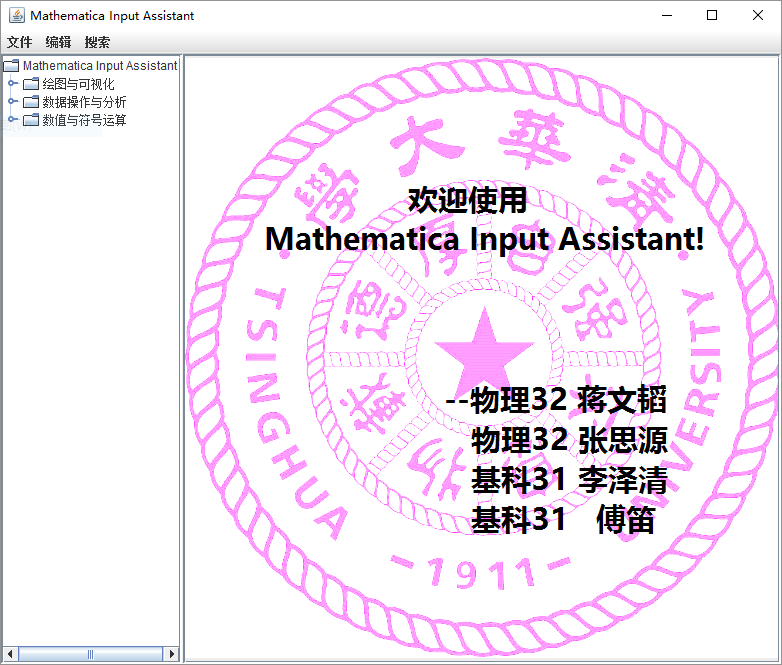
\includegraphics[width=4in]{1.png}
                	\caption{欢迎界面测试}    
                	\label{pic:MathObject}
            	\end{figure}

		\end{itemize}
		
		% subsection 欢迎界面测试_ (end)

		\subsection{菜单栏子目录显示、左侧树形结构窗口按钮以及滚动条使用测试} % (fold)
		\begin{itemize}
			\item 用例名称: 菜单栏子目录显示、左侧树形结构窗口按钮以及滚动条使用测试
			\item 用例描述: 点击节点以及菜单栏按钮,右侧欢迎界面不发生变化,点击函数函数类文件或文件夹,右侧进入对应函数函数类的操作界面。
			\item 测试过程: 单击节点、菜单栏按钮以及函数函数类文件和文件夹。
			\item 预计结果: 按照用例描述,右侧界面对应发生变化。
			\item 测试结果:	和预期结果相一致。

				\begin{figure}[!h]
	                \begin{minipage}[b]{0.45\textwidth}
	                \centering
	                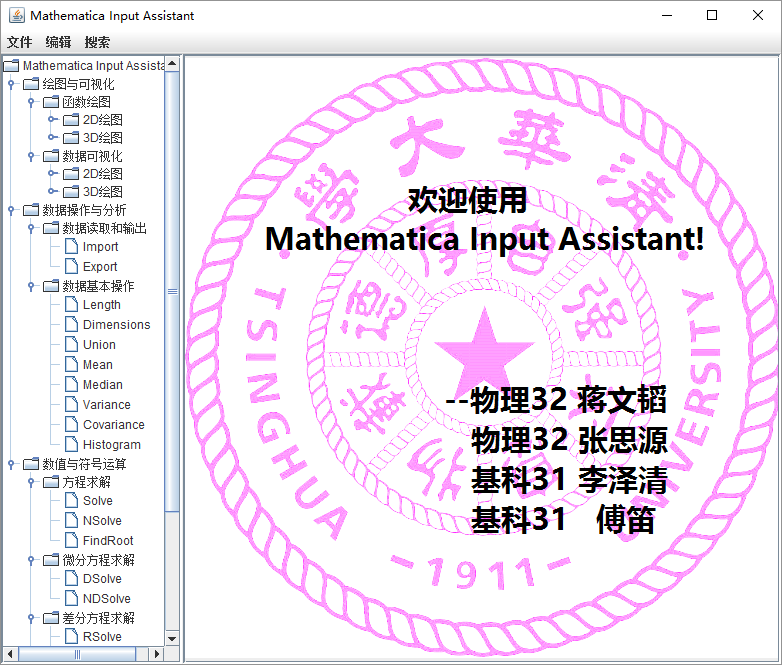
\includegraphics[width=3in]{2.png}
	                \caption{展开树节点}
	                \label{pic:MathPack}
	                \end{minipage}%
	                \hspace{0.1\textwidth}%
	                \begin{minipage}[b]{0.45\textwidth}
	                \centering
	                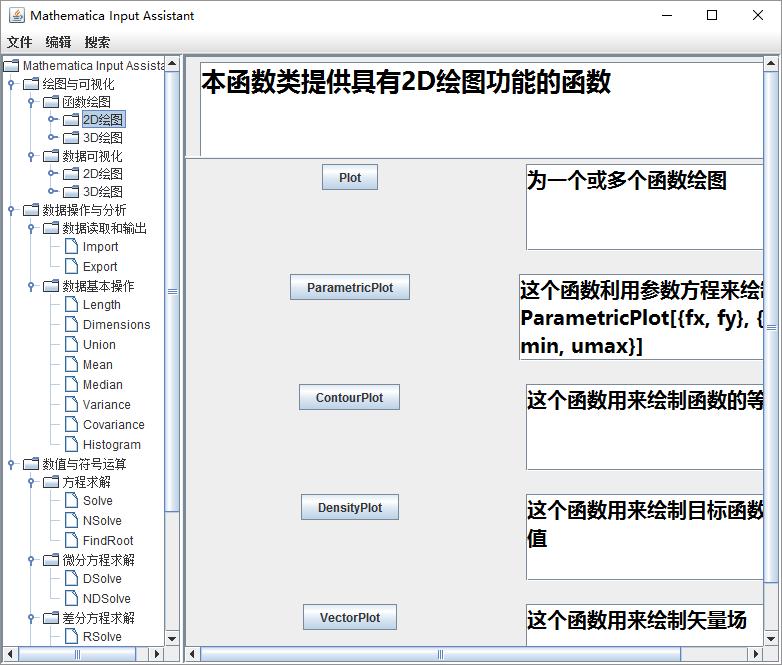
\includegraphics[width=3in]{3.png}
	                \caption{进入函数函数类操作界面}
	                \label{pic:GUIPack}
	                \end{minipage}
            	\end{figure}

		\end{itemize}
		
		
		% subsection 菜单栏子目录显示_左侧树形结构窗口按钮以及滚动条使用测试 (end)
	
	% section 表观测试 (end)

		\subsection{子对话框的显示} % (fold)
		\begin{itemize}
			\item 用例名称: 子对话框的显示
			\item 用例描述: 点击菜单栏按钮下拉菜单内的选项,正确弹出所需对话框。
			\item 测试过程: 单击菜单栏下拉菜单中各个按钮。
			\item 预计结果: 按照用例描述,正确显示所需子对话框。
			\item 测试结果:	和预期结果相一致。

				\begin{figure}[!h]
                	\centering
                	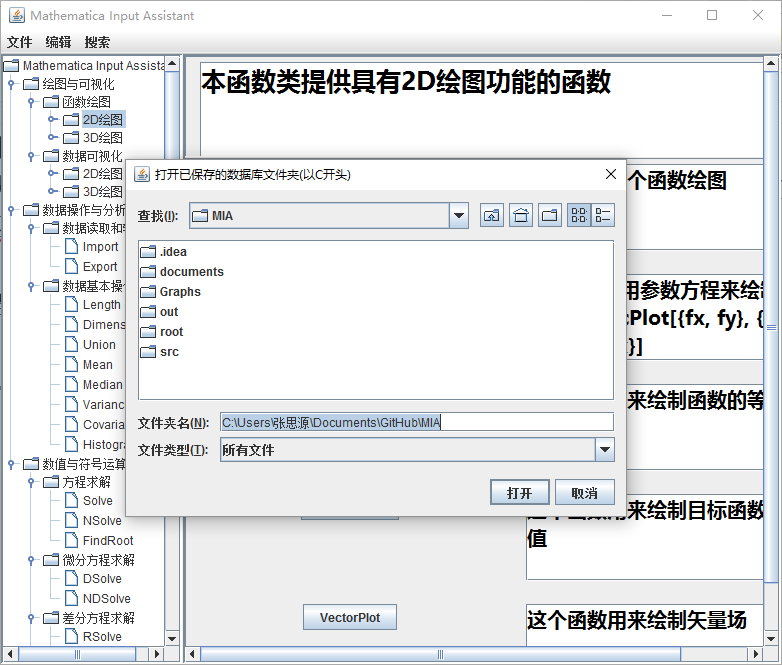
\includegraphics[width=4in]{4.png}
                	\caption{子对话框的显示}    
                	\label{pic:MathObject}
            	\end{figure}

		\end{itemize}
	
	% subsection 子对话框的显示 (end)section{子对话框的显示} % (fold)
	
		\subsection{右侧操作窗口按钮测试} % (fold)
		\begin{itemize}
			\item 用例名称: 右侧操作窗口按钮测试
			\item 用例描述: 点击右侧窗口按钮也可以进入对应函数或函数类。
			\item 测试过程: 单击Parametric Plot按钮进入Parametric Plot操作和介绍界面。
			\item 预计结果: 按照用例描述,正确进入Parametric Plot操作介绍界面,其他按钮同样进行测试。
			\item 测试结果:	和预期结果相一致。

				\begin{figure}[!h]
                	\centering
                	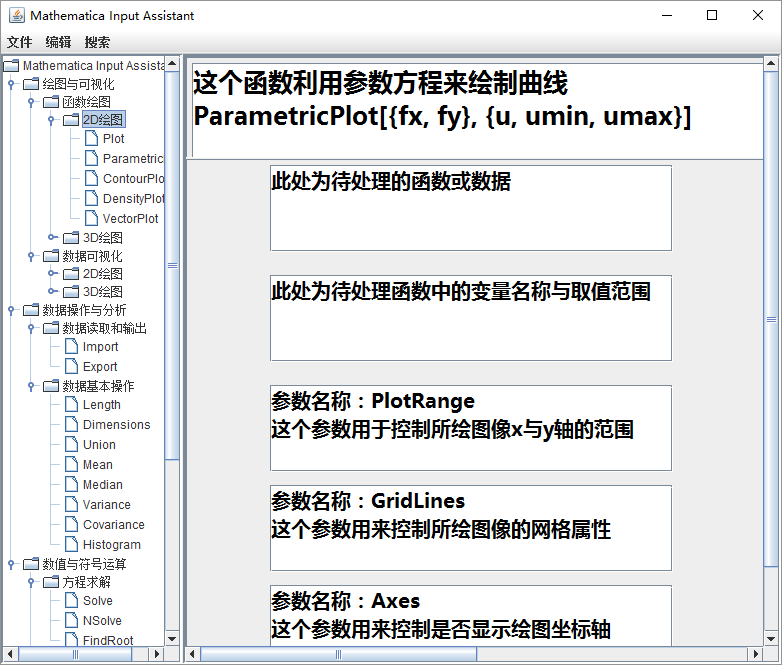
\includegraphics[width=4in]{5.png}
                	\caption{右侧操作窗口按钮测试}    
                	\label{pic:MathObject}
            	\end{figure}

		\end{itemize}
	
	% subsection 右侧操作窗口按钮测试 (end)

	\section{函数使用测试} % (fold)
		\subsection{ParametricPlot} % (fold)
		\begin{itemize}
			\item 用例名称: ParametricPlot
			\item 用例描述: 在右侧上面部分按照提示进行输入和选择,点击生成代码然后拷入Mathematica中运行,显示所要画图功能。
			\item 测试过程: 按照图示输入,单击生成代码,拷入Mathematica运行。
			\item 预计结果: 按照用例描述,正确显示参数图像。
			\item 测试结果:	和预期结果相一致。

				\begin{figure}[!h]
	                \begin{minipage}[b]{0.45\textwidth}
	                \centering
	                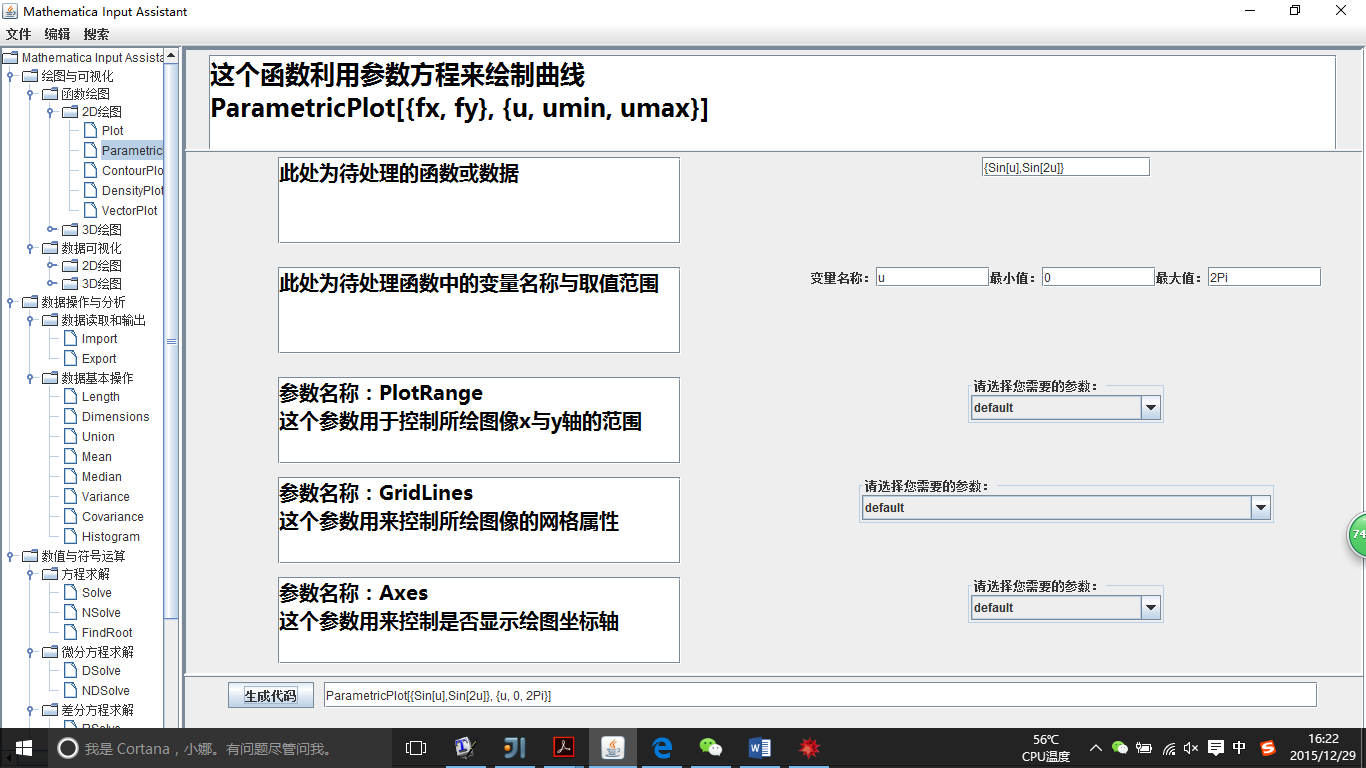
\includegraphics[width=3in]{6.png}
	                \caption{按提示进行输入和选择生成代码}
	                \label{pic:MathPack}
	                \end{minipage}%
	                \hspace{0.1\textwidth}%
	                \begin{minipage}[b]{0.45\textwidth}
	                \centering
	                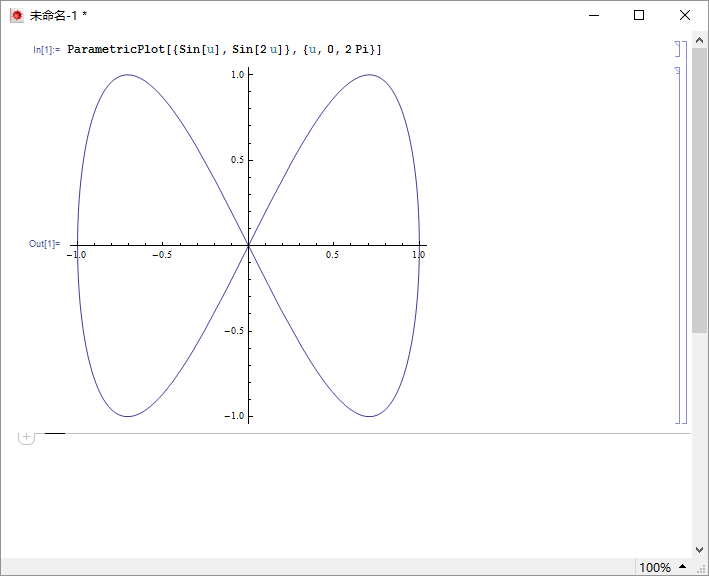
\includegraphics[width=3in]{7.png}
	                \caption{拷入Mathematica中运行}
	                \label{pic:GUIPack}
	                \end{minipage}
            	\end{figure}

		\end{itemize}
		
		% subsection parametricplot (end)
		
		\subsection{ContourPlot3D} % (fold)
		\begin{itemize}
			\item 用例名称: ContourPlot3D
			\item 用例描述: 在右侧上面部分按照提示进行输入和选择,点击生成代码然后拷入Mathematica中运行,显示所要画图功能。
			\item 测试过程: 按照图示输入,单击生成代码,拷入Mathematica运行。
			\item 预计结果: 按照用例描述,正确显示参数图像。
			\item 测试结果:	和预期结果相一致。

				\begin{figure}[!h]
	                \begin{minipage}[b]{0.45\textwidth}
	                \centering
	                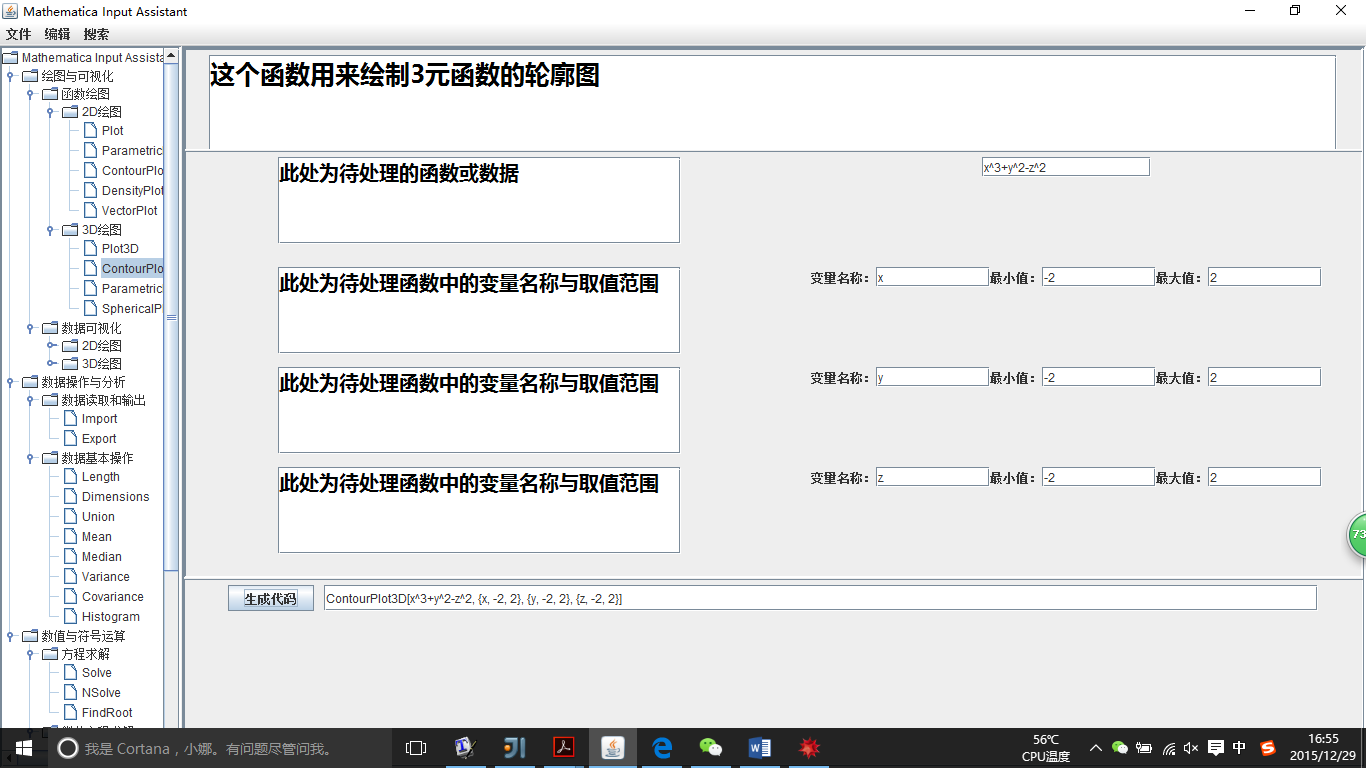
\includegraphics[width=3in]{8.png}
	                \caption{按提示进行输入和选择生成代码}
	                \label{pic:MathPack}
	                \end{minipage}%
	                \hspace{0.1\textwidth}%
	                \begin{minipage}[b]{0.45\textwidth}
	                \centering
	                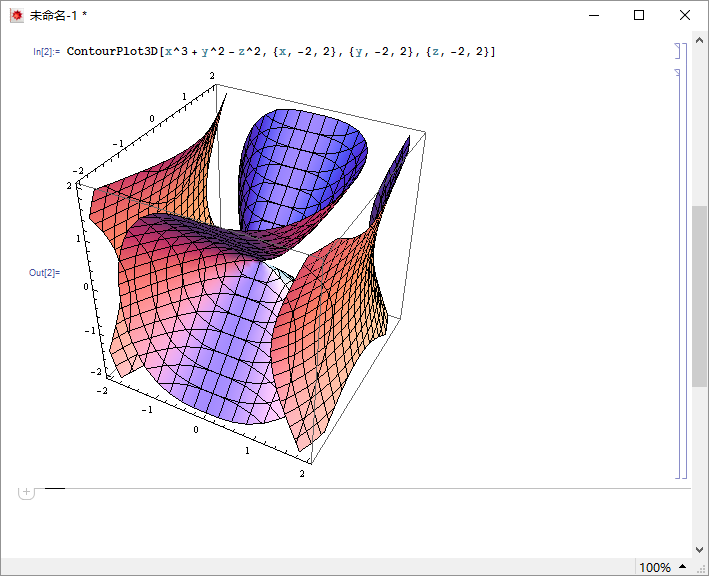
\includegraphics[width=3in]{9.png}
	                \caption{拷入Mathematica中运行}
	                \label{pic:GUIPack}
	                \end{minipage}
            	\end{figure}

		\end{itemize}
		
		% subsection contourplot3d (end)

		\subsection{其它} % (fold)
		其他部分已经实现函数也进行了测试,和预期结果基本一致。
		
		% subsection 其它 (end)
	
	% section 函数使用测试 (end)

	\section{函数和函数类添加测试} % (fold)
		\begin{itemize}
			\item 用例名称: PolarPlot
			\item 用例描述: 首先在菜单栏选择添加函数进一步添加参数和自变量取值范围,如图输入,在右侧上面部分按照提示进行输入和选择,点击生成代码然后拷入Mathematica中运行,显示所要画图功能。
			\item 测试过程: 按图添加函数以及函数Axes参数以及自变量取值范围,按照图示输入,单击生成代码,拷入Mathematica运行。
			\item 预计结果: 按照用例描述,正确显示参数图像。
			\item 测试结果:	和预期结果相一致。

				\begin{figure}[!h]
	                \begin{minipage}[b]{0.45\textwidth}
	                \centering
	                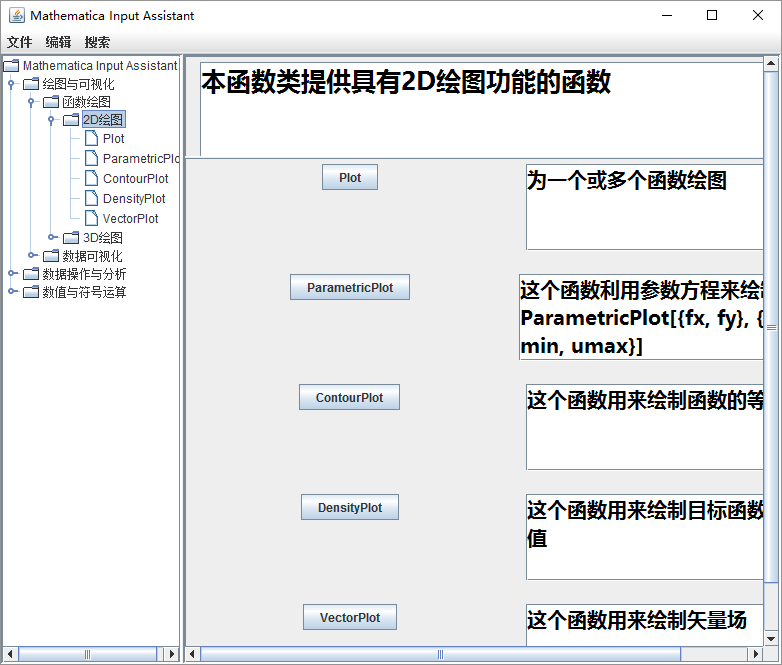
\includegraphics[width=3in]{10.png}
	                \caption{选择添加函数所在函数类}
	                \label{pic:MathPack}
	                \end{minipage}%
	                \hspace{0.1\textwidth}%
	                \begin{minipage}[b]{0.45\textwidth}
	                \centering
	                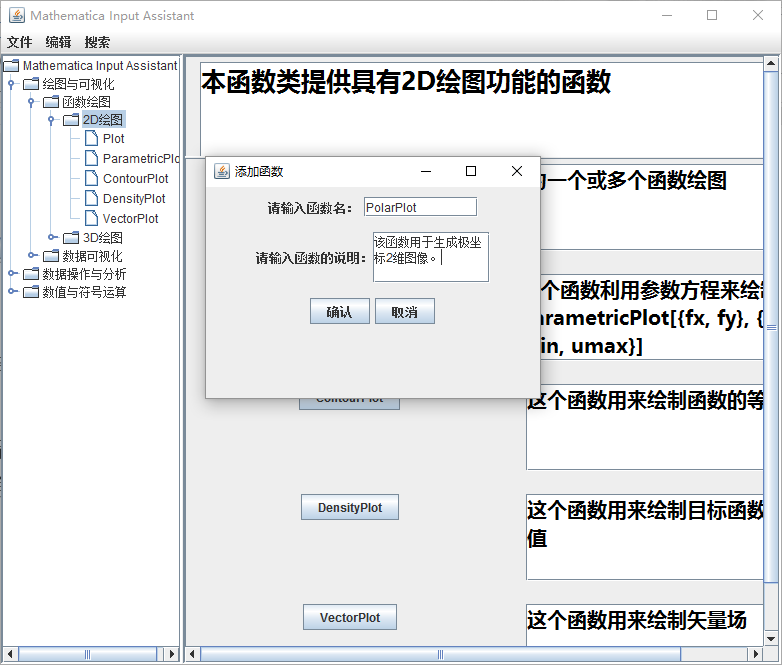
\includegraphics[width=3in]{11.png}
	                \caption{选择添加函数}
	                \label{pic:GUIPack}
	                \end{minipage}
            	\end{figure}

            	\begin{figure}[!h]
	                \begin{minipage}[b]{0.45\textwidth}
	                \centering
	                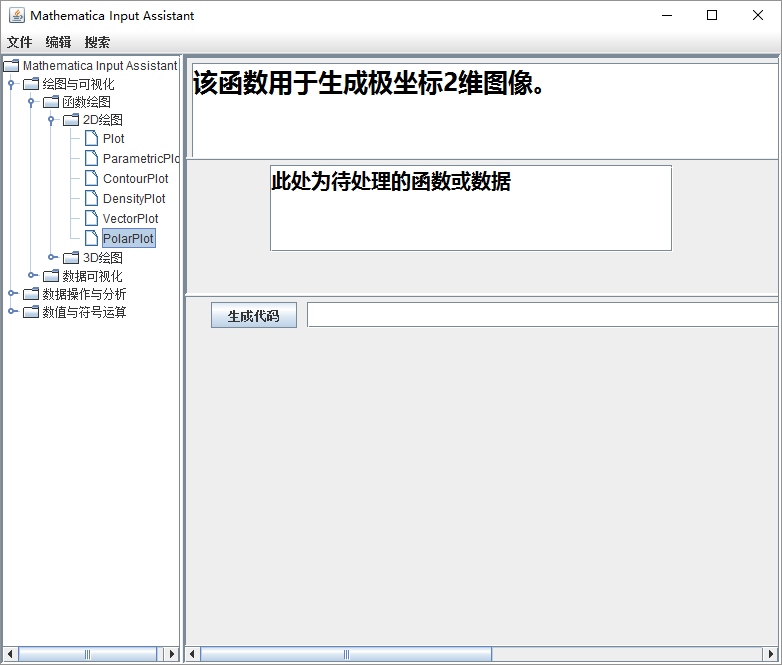
\includegraphics[width=3in]{12.png}
	                \caption{显示所添加函数}
	                \label{pic:MathPack}
	                \end{minipage}%
	                \hspace{0.1\textwidth}%
	                \begin{minipage}[b]{0.45\textwidth}
	                \centering
	                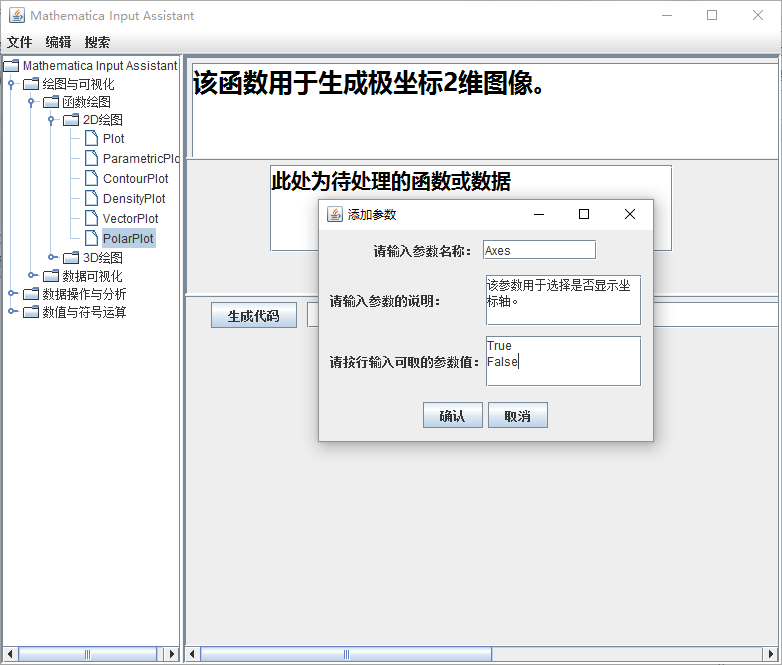
\includegraphics[width=3in]{13.png}
	                \caption{添加参数}
	                \label{pic:GUIPack}
	                \end{minipage}
            	\end{figure}

            	\begin{figure}[!h]
	                \begin{minipage}[b]{0.45\textwidth}
	                \centering
	                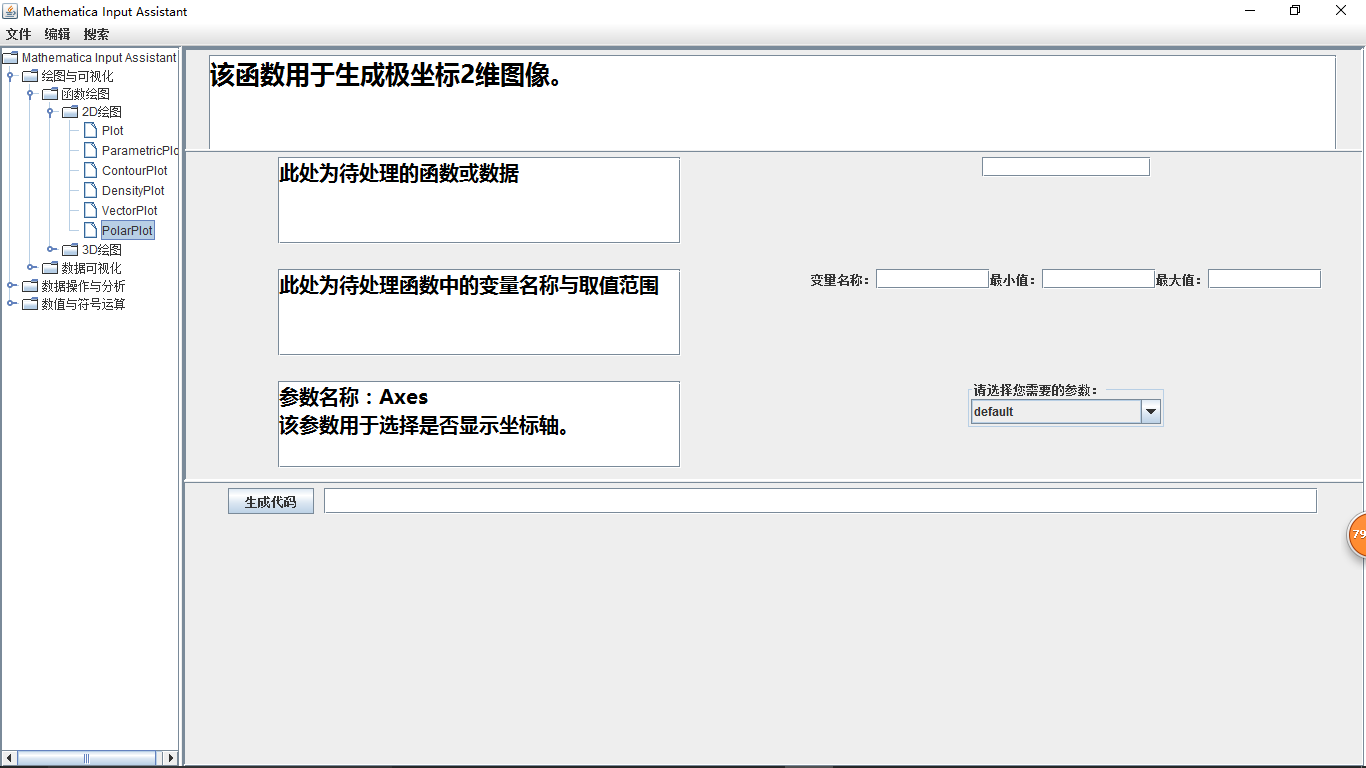
\includegraphics[width=3in]{14.png}
	                \caption{添加自变量取值范围}
	                \label{pic:MathPack}
	                \end{minipage}%
	                \hspace{0.1\textwidth}%
	                \begin{minipage}[b]{0.45\textwidth}
	                \centering
	                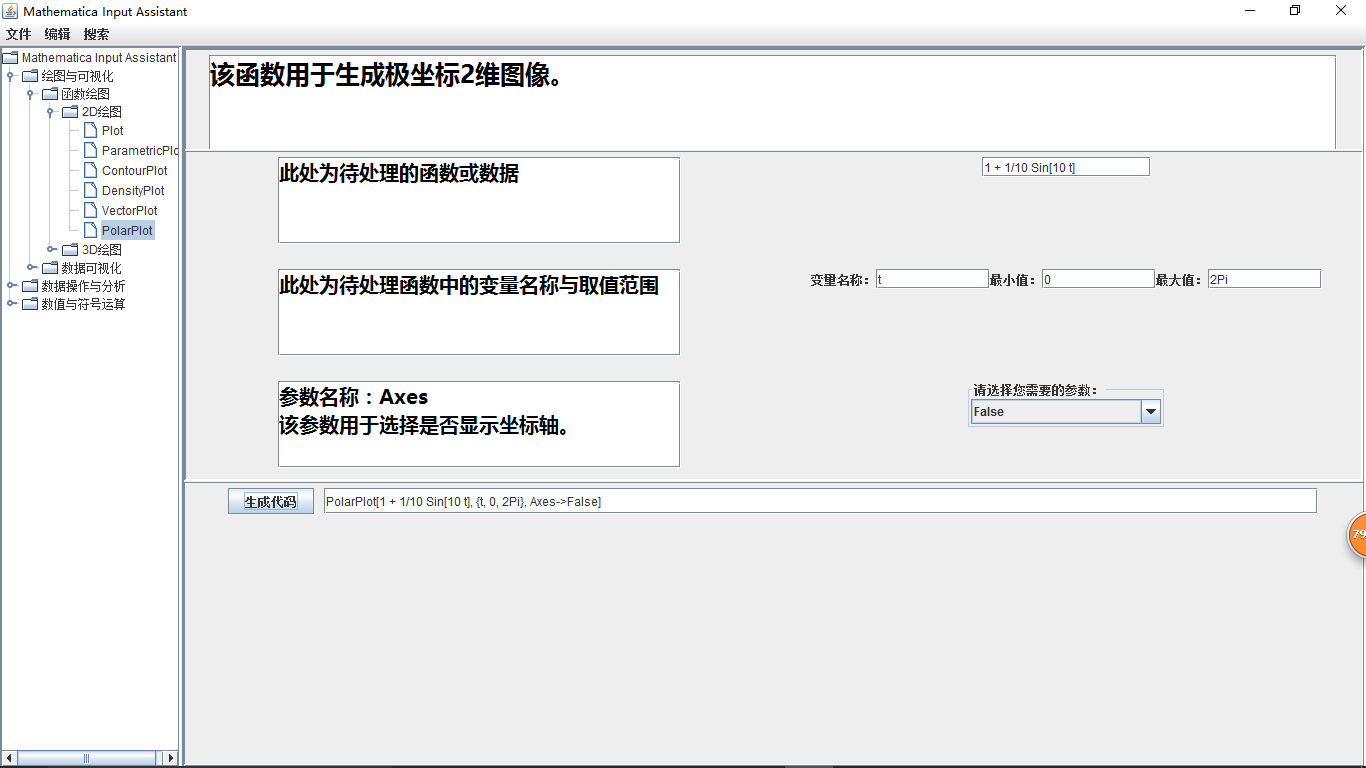
\includegraphics[width=3in]{15.png}
	                \caption{按图输入}
	                \label{pic:GUIPack}
	                \end{minipage}
            	\end{figure}

            	\begin{figure}[!h]
                	\centering
                	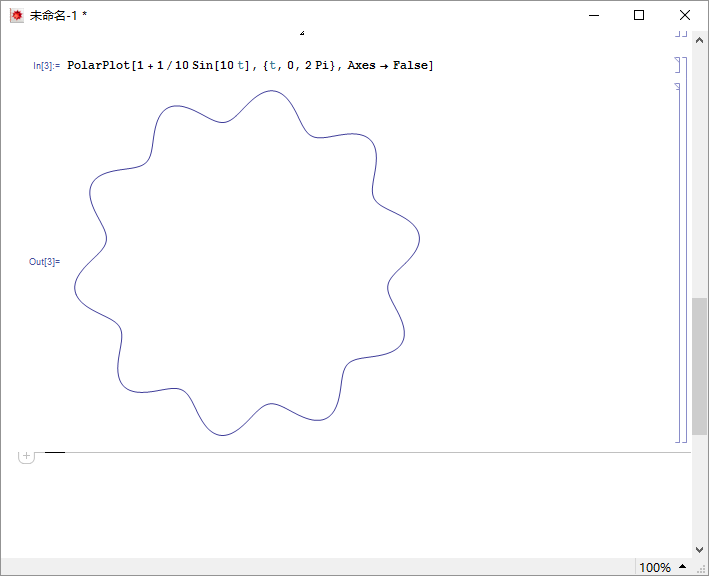
\includegraphics[width=4in]{16.png}
                	\caption{拷入Mathematica中运行}    
                	\label{pic:MathObject}
            	\end{figure}

		\end{itemize}

	% section 函数和函数类添加测试 (end)

	\section{搜索函数功能测试} % (fold)
		\subsection{搜索框弹出测试} % (fold)
		\begin{itemize}
			\item 用例名称: 搜索框弹出测试
			\item 用例描述: 点击菜单栏搜索按钮,弹出搜索对话框。
			\item 测试过程: 单击菜单栏搜索按钮,观测是否正确弹出搜索对话框。
			\item 预计结果: 按照用例描述,正确显示搜索对话框。
			\item 测试结果:	和预期结果相一致。

				\begin{figure}[!h]
                	\centering
                	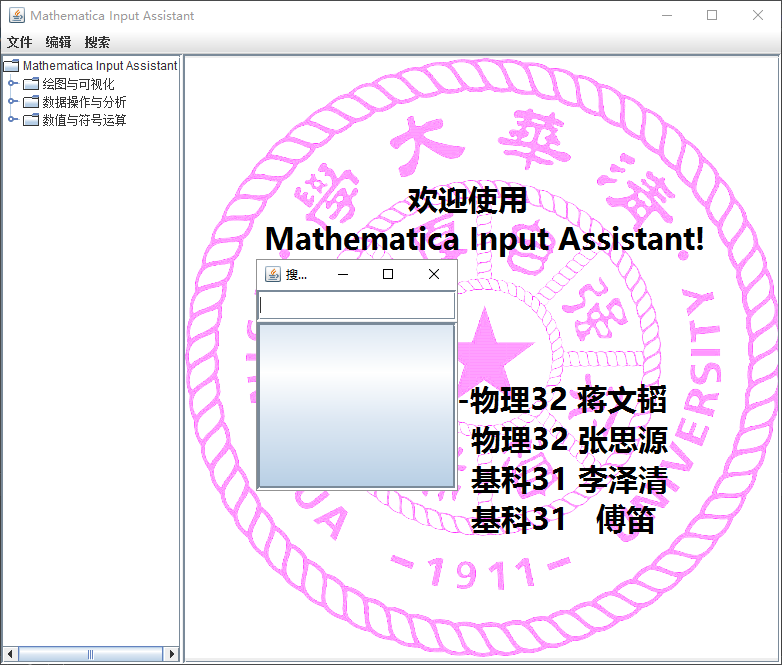
\includegraphics[width=4in]{17.png}
                	\caption{搜索框弹出测试}    
                	\label{pic:MathObject}
            	\end{figure}

		\end{itemize}
		% subsection 搜索框弹出测试 (end)

		\subsection{即时反应检索功能测试} % (fold)
		\begin{itemize}
			\item 用例名称: 即时反应检索功能测试
			\item 用例描述: 点击菜单栏搜索按钮,弹出搜索对话框。
			\item 测试过程: 输入p,搜索对话框如图显示;再输入l后,搜索对话框变化如图显示。
			\item 预计结果: 按照用例描述,正确即时更新搜索结果。
			\item 测试结果:	和预期结果相一致。

				\begin{figure}[!h]
	                \begin{minipage}[b]{0.45\textwidth}
	                \centering
	                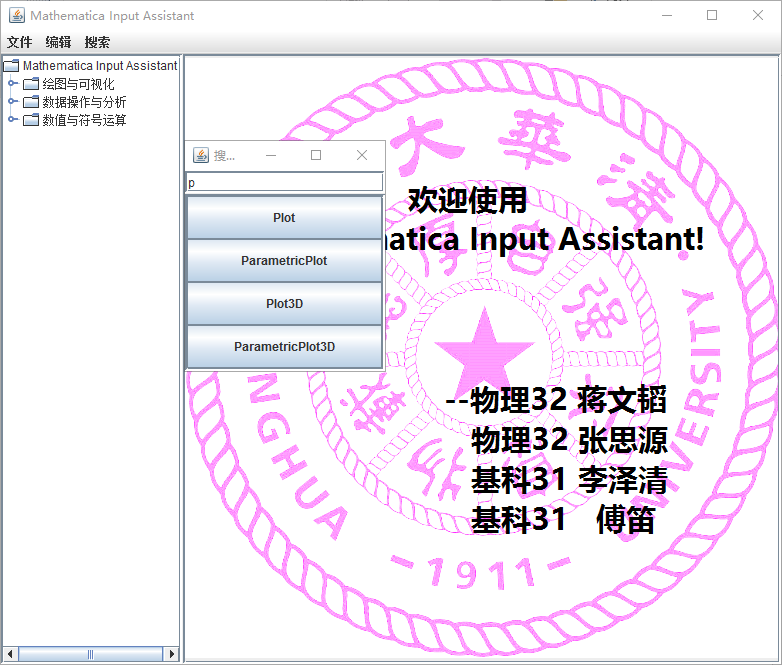
\includegraphics[width=3in]{18.png}
	                \caption{输入p}
	                \label{pic:MathPack}
	                \end{minipage}%
	                \hspace{0.1\textwidth}%
	                \begin{minipage}[b]{0.45\textwidth}
	                \centering
	                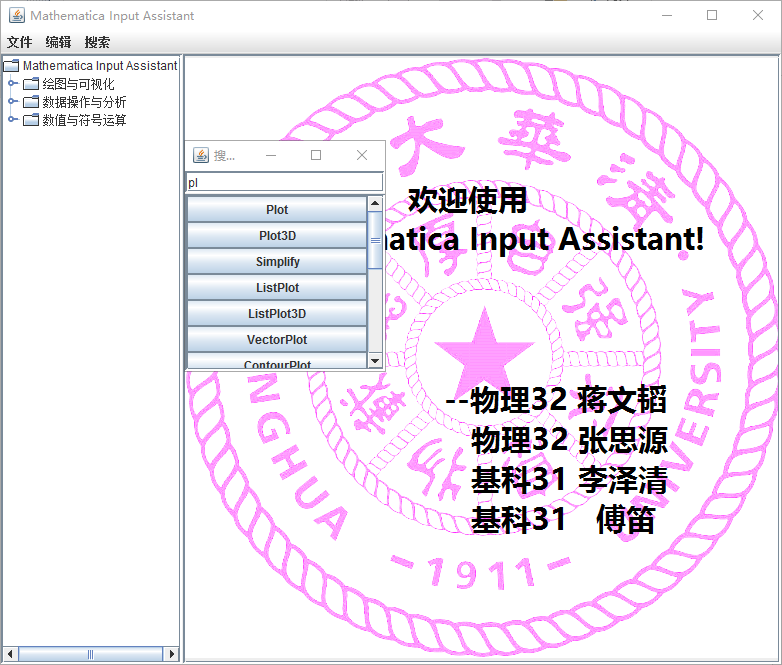
\includegraphics[width=3in]{19.png}
	                \caption{再输入l}
	                \label{pic:GUIPack}
	                \end{minipage}
            	\end{figure}

		\end{itemize}
		
		% subsection 即时反应检索功能测试 (end)

		\subsection{搜索对话框按钮测试} % (fold)
		\begin{itemize}
			\item 用例名称: 搜索对话框按钮测试
			\item 用例描述: 点击搜索对话框函数按钮,主界面右侧进入对应函数操作界面。
			\item 测试过程: 单击Plot3D按钮,搜索对话框消失,并且主界面对Plot3D函数操作界面给予显示。
			\item 预计结果: 按照用例描述,正确显示。
			\item 测试结果:	和预期结果相一致。

				\begin{figure}[!h]
                	\centering
                	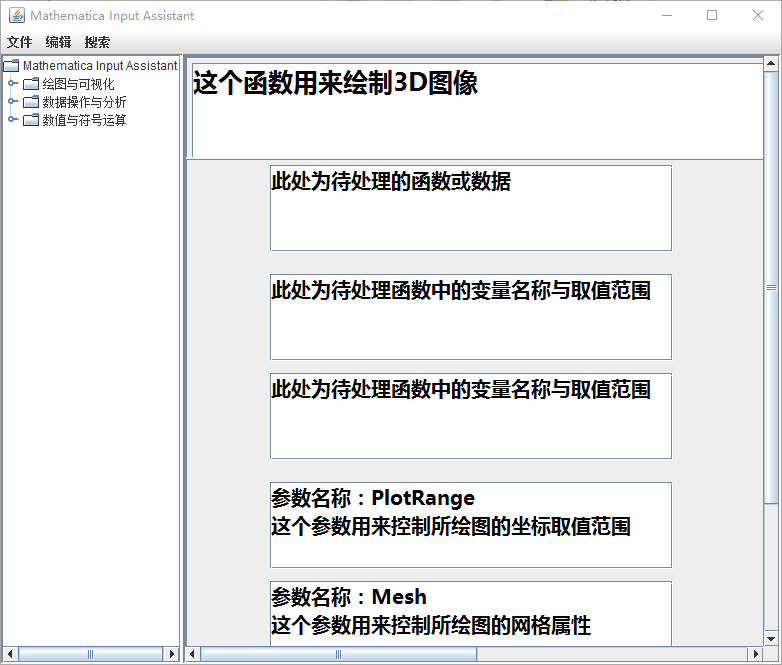
\includegraphics[width=4in]{20.png}
                	\caption{搜索对话框按钮测试}    
                	\label{pic:MathObject}
            	\end{figure}

		\end{itemize}
		
		% subsection 搜索对话框按钮测试 (end)
	
	% section 搜索函数功能测试 (end)

	\section{细节功能测试} % (fold)
		\subsection{函数名称输入非法测试} % (fold)
		如果函数名称输入非字母符号是不合法的,将会自动报错。
		\begin{figure}[!h]
	        \begin{minipage}[b]{0.45\textwidth}
	        \centering
	        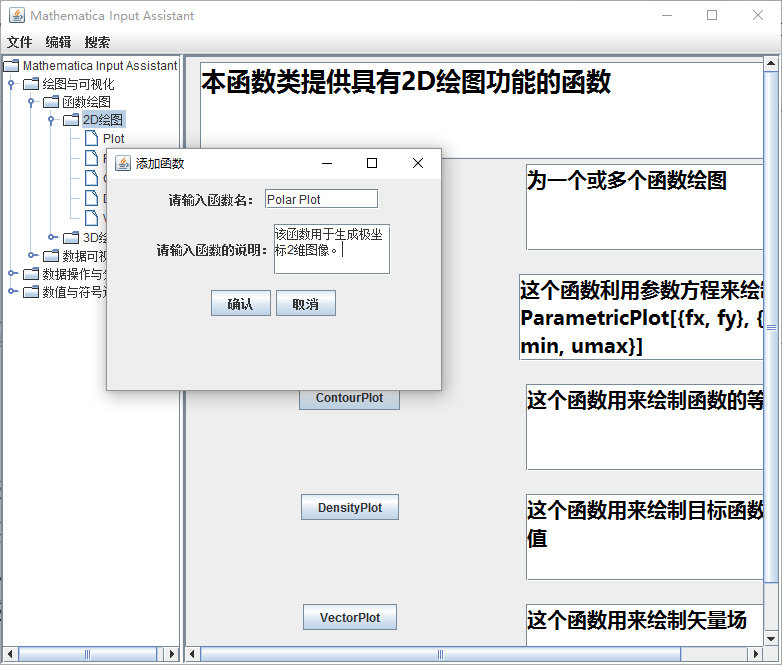
\includegraphics[width=3in]{22.png}
	        \caption{输入非法字符}
	        \label{pic:MathPack}
	        \end{minipage}%
	        \hspace{0.1\textwidth}%
	        \begin{minipage}[b]{0.45\textwidth}
	        \centering
	        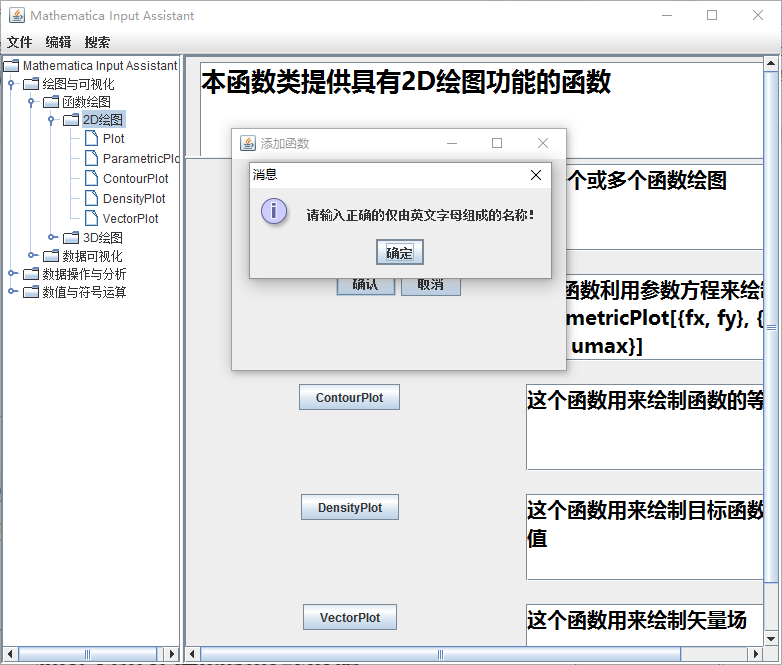
\includegraphics[width=3in]{21.png}
	        \caption{提示报错}
	        \label{pic:GUIPack}
	        \end{minipage}
        \end{figure}
		
		% subsection 函数名称输入非法测试 (end)

		\subsection{步长选择提示} % (fold)
		\begin{figure}[!h]
           	\centering
           	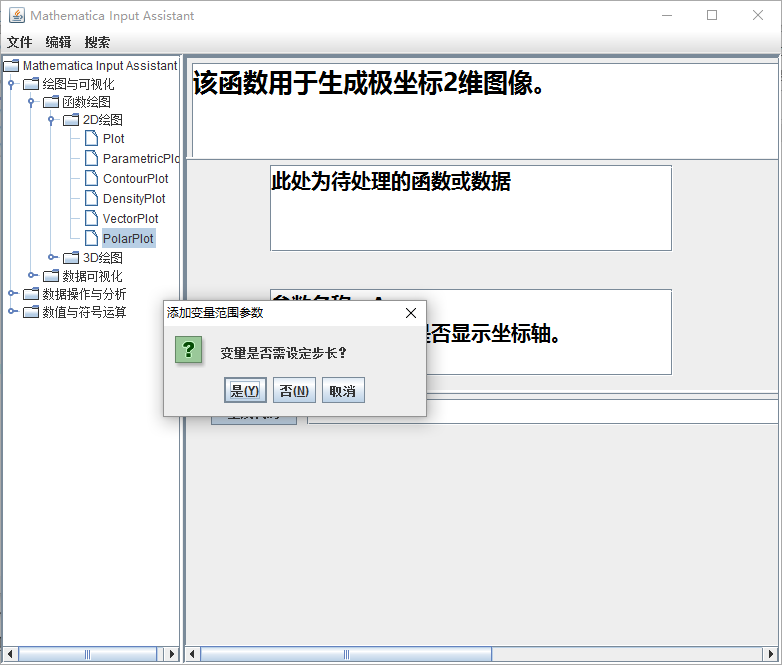
\includegraphics[width=4in]{23.png}
           	\caption{步长选择提示}    
           	\label{pic:MathObject}
        \end{figure}
		
		% subsection 步长选择提示 (end)

		\subsection{函数函数类删除操作} % (fold)
		能够正确删除函数和函数类,并且退回欢迎界面。
		\begin{figure}[!h]
	        \begin{minipage}[b]{0.45\textwidth}
	        \centering
	        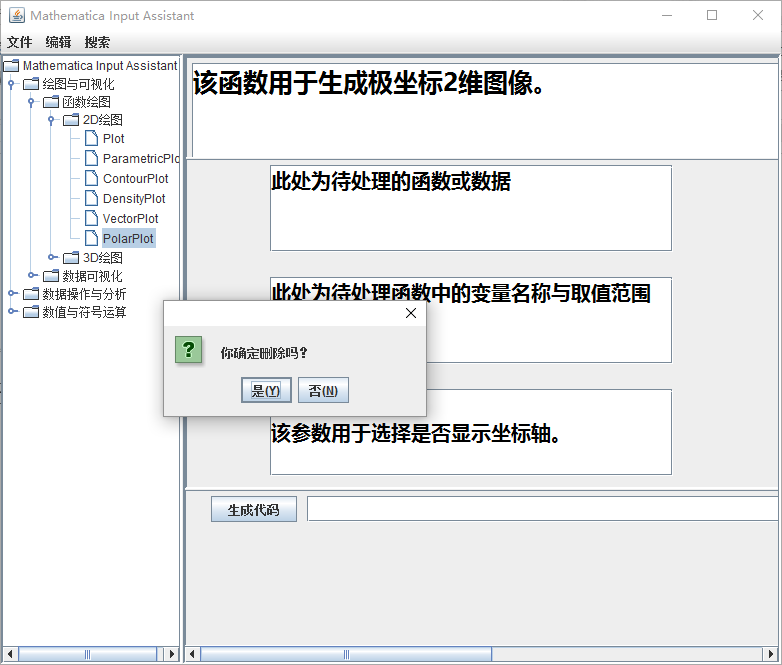
\includegraphics[width=3in]{24.png}
	        \caption{再次询问是否删除函数}
	        \label{pic:MathPack}
	        \end{minipage}%
	        \hspace{0.1\textwidth}%
	        \begin{minipage}[b]{0.45\textwidth}
	        \centering
	        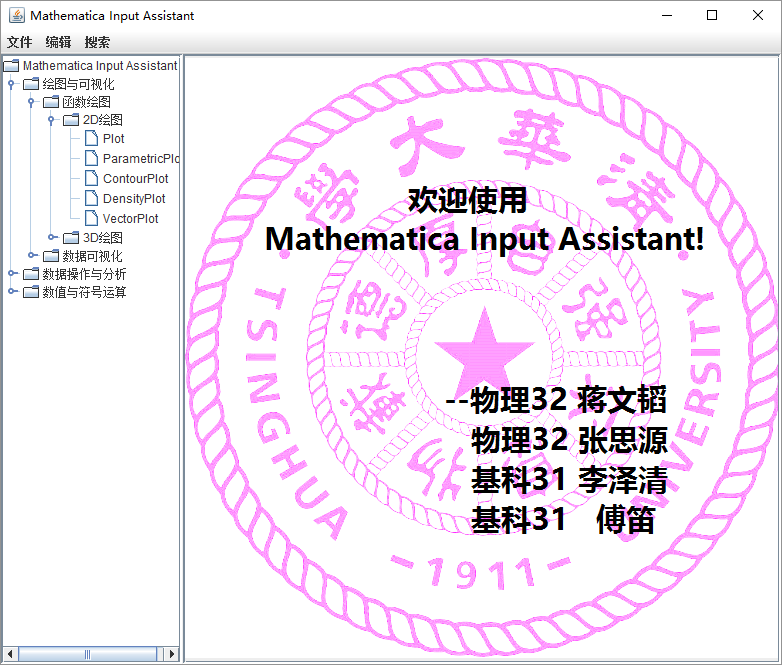
\includegraphics[width=3in]{25.png}
	        \caption{删除函数返回欢迎界面}
	        \label{pic:GUIPack}
	        \end{minipage}
        \end{figure}
		
		% subsection 函数删除操作 (end)

		\subsection{其它} % (fold)
		如果不点击保存,则下次打开文件后,之前添加的函数就不会显示,保存之后就可以显示。
		
		% subsection 其它 (end)
	
	% section 细节功能测试 (end)

\chapter{测试结果及改进}

	\section{测试结果} % (fold)
	所有测试均通过测试。
	
	% section 测试结果 (end)

	\section{测试改进} % (fold)
	界面可以进一步优化;另外已有函数描述可以进一步优化,以更加方便初学者使用Mathematica。
	
	% section 测试改进 (end)

\end{document}